\documentclass[conference]{IEEEtran}
\IEEEoverridecommandlockouts
% The preceding line is only needed to identify funding in the first footnote. If that is unneeded, please comment it out.
\usepackage{cite}
\usepackage{amsmath,amssymb,amsfonts}
\usepackage{algorithmic}
\usepackage{graphicx}
\usepackage{textcomp}
\usepackage{xcolor}
\def\BibTeX{{\rm B\kern-.05em{\sc i\kern-.025em b}\kern-.08em
    T\kern-.1667em\lower.7ex\hbox{E}\kern-.125emX}}
\begin{document}

\title{Conference Paper Title*\\
{\footnotesize \textsuperscript{*}Note: Sub-titles are not captured in Xplore and
should not be used}
\thanks{Identify applicable funding agency here. If none, delete this.}
}

\author{\IEEEauthorblockN{ Benedikt Lipinski}
\IEEEauthorblockA{\textit{Hochschule Hamm- Lippstadt} \\
Soest,Germany \\
benedikt.lipinski@stud.hshl.de}
\and
\IEEEauthorblockN{ Jonas Gerken}
\IEEEauthorblockA{\textit{dept. name of organization (of Aff.)} \\
\textit{name of organization (of Aff.)}\\
City, Country \\
email address or ORCID}
\and
\IEEEauthorblockN{ Michael Jathe}
\IEEEauthorblockA{\textit{dept. name of organization (of Aff.)} \\
\textit{name of organization (of Aff.)}\\
City, Country \\
email address or ORCID}
\and
\IEEEauthorblockN{ Niklas Heiber}
\IEEEauthorblockA{\textit{dept. name of organization (of Aff.)} \\
\textit{name of organization (of Aff.)}\\
City, Country \\
email address or ORCID}

}

\maketitle

\begin{center}
\begin{abstract}
This document is a model and instructions for \LaTeX.
This and the IEEEtran.cls file define the components of your paper [title, text, heads, etc.]. *CRITICAL: Do Not Use Symbols, Special Characters, Footnotes, 
or Math in Paper Title or Abstract.
\end{abstract}
\end{center}
\titlepage

\section{Motivation (BL)}
In Katastrophenlagen und Ausnahmesituationen können für Menschen oft lebensbedrohliche Bedingungen herrschen. So, dass es im Einsatz von Rettungskräften nicht selten zu gefährlichen Momenten kommt, in denen die eigentlich zur Hilfe eingesetzten Kräfte, selbst zu Hilfe-Ersuchenden werden. \par
Ein Einsatzszenario, in dem Verletzungen, oft schwerwiegend sind, ist die Bedrohung durch Waldbrände. Das Risiko für Einsatzkräfte, sich bei einem Waldbrand zu verletzten, steigt mit jedem brennenden Hektar an Fläche deutlich an. So zeigte sich hier in den letzten 2 Jahren ein starker Anstieg an brennender Fläche mit zuletzt im Jahr 2019 2.711 ha Fläche \cite[S.7B1]{stat1}. Da ein Anstieg an brennender Fläche nicht nur ein erhöhtes Verletzungsrisiko, sondern auch erschwerte Bedingungen an die Einsatzdurchführung selbst stellt. \par
Da der Schutz von Menschenleben und Einsatzkräften an oberste Stelle steht, aber die Bedingungen in einem Waldbrandeinsatz nicht immer den gedankenlosen Einsatz von menschlichem Personal zulassen, sind die rettenden Einheiten auf technische Lösungen angewiesen, die zu ihrem Schutz und ihrer Unterstützung beitragen.\par 
Zur schnelleren Rettung von vermissten Personen und gleichzeitigem Selbstschutz von Einsatzkräften wird ein technisches Gerät benötigt, das verletzte Personen in einem Waldbrandgebiet aufsuchen kann und somit eine Rettung der Person ohne Gefahr für dritte bezweckt. 
Entwickelt werden soll ein Prototyp, der automatisiert und selbständig eine verletzte Person in einer vorgegeben Umgebung aufspüren kann(A). Der Roboter kann sowohl über Land, wie auch über Wasser zu seinem Ziel gelangen(A1,A2), was ihm mittels eines Kettenantriebes ermöglicht wird(A1.1). Damit das Fahren auf dem Wasser möglich ist, werden an den Laufwerken einzelne Kettenglieder zu Paddelblechen geformt (A2.3)
Um sich selbstständig in seiner Umgebung zurechtfinden zu können, muss der Roboter Hindernisse erkennen und ihnen ausweichen können(A3,A3.1).
\par Um sich im Gelände orientieren zu können, navigiert sich der Roboter indem er auf ein spezifisch codiertes Schall-Signal von bis zu 4 Türmen reagieren kann (C, C.1)
In der Interaktion mit einem potentiellen Waldbrandopfer soll das Fahrzeug einen Ersthilfekasten bei sich tragen(B), um der gefundenen Person zu ermöglichen, kleinere Verletzungen bei sich selbst zu behandeln. Zudem sollen Temperaturen von Objekten bestimmt werden können, damit die eines Menschen so wie auch die Temperatur des zu befahrenen Bereichs bestimmt werden kann ( D.1). Des Weiteren kann die verletzte Person mittels einer Gegensprechanlage Kontakt mit dem Rettungspersonal aufnehmen(E). Eine weitere- jedoch verworfene- Anforderung ist die Entscheidung für einen Landweg, sollte das Fahrzeug zu schwer gelastet sein. Jedoch sind im Projektverlauf weitere Anforderungen hinzu gekommen, zum Beispiel wäre das die Umsetzung einer vom Operator per Fernbedienung gesteuerten Kettensäge auf dem Roboter. Diese Funktion soll eine bessere Fortbewegung im Gelände ermöglichen.
\par Die Anforderungen wurden durch die komplette Gruppe anhand des durch die Aufgabe festgelegten Rahmens erstellt.

\begin{figure}[h] 
\center{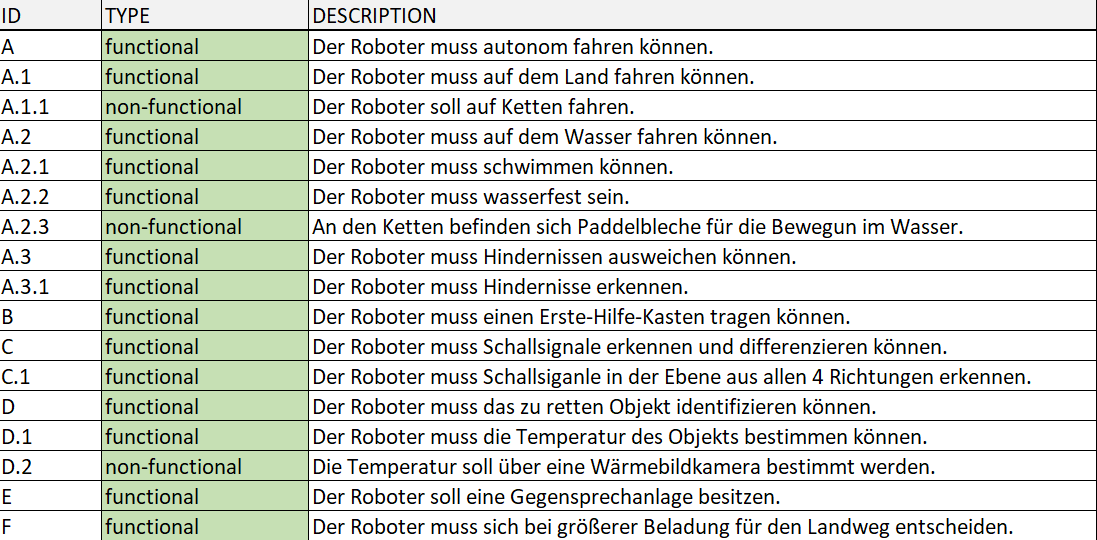
\includegraphics[scale=0.3]{Requirements}}
\caption{Anforderungsliste }
\label{fig.1}
\end{figure}





\section{Implementation des Roboters (BL)}
{
Als letzten Schritt vor der finalen Umsetzung in wirklichen Programmiercode wurden die abgeleiteten Algorithmen beispielhaft ohne jegliche reale Syntax Umgesetzt. Die diente zum besseren Verständnis der späteren Übersetzung der Algorithmen von der Beschreibung durch Diagramme in die Beschreibung durch von Maschinen lesbare Sprache. Ziel war es zudem, nicht nur einem Compiler die Lesbarkeit zu ermöglichen, sondern auch die Abstimmung in der Gruppe, um zu gewährleisten, dass der durch mich abgeleitete Code, auch den übrigen Gruppenmitgliedern in der Form schlüssig erschien und nicht durch ein Verständnisproblem in eine falsche Richtung entwickelt wurde. Ein positiver Nebeneffekt ist zudem, dass sich bereits nach der Umsetzung in Pseudo-Code mögliche Unstimmigkeiten in Schnittstellen aufgetan hätten, aber auch die Arbeit von mehr als einer Person in der weiteren Umsetzung nicht die Gefahr gebracht hätte, Fehler zu erzeugen. \par
Die Entscheidung, in welcher Programmiersprache der Roboter umgesetzt wird, fiel auf C++. Die Gründe für die Auswahl ergeben sich daraus, dass Programme in C++ leicht zu verstehen und auch umzusetzen sind. Das bedeutet, die Programmierung war für alle Teilnehmer in der Gruppe ohne Probleme möglich, da bereits im Verlauf des Studiums alle Mitglieder mehrfach durch die Arduino-Programmierung im Rahmen von Projekten zu tun hatten und somit nicht erst eine neue Sprache zu erlernen hatten. Weitere Vorteile von C++ sind, dass die Sprache in ihrem Kern recht schlank ist, und somit sehr schlank ist. Auf Funktionen muss allerdings nicht verzichtet werden, da eine große Anzahl an Bibliotheken zur Verfügung steht, die bei Bedarf mit eingebunden werden können. Letzter Entscheidungsgrund für C++ ist der Schlankheit der Sprache geschuldet. Entscheidend war der Faktor, dass C++ auf einer hohen Anzahl an Umgebungen zur Verfügung steht. Beispiele wären der bereits erwähnte Arduino, der sich besonders für das Entwickeln von Prototypen eignet. Ein weiteres Beispiel sind Microsoft Windows Betriebssysteme, in denen mit einem C++ Compiler und den Entwicklungsumgebungen von zum Beispiel  Visual Studio oder Eclipse sehr komfortabel Quellcode in C++ entwickelt werden kann.\par 
Zu den aktuellen Bestandteilen des Systems, die in Programmiercode umgesetzt wurden, zählen die elementaren Bestandteile der selbständigen Fahrt zu einer verunfallten Person in einem Testszenario. Genauer wurde die Entscheidung umgesetzt, ob ein Fahrzeug sich zum Zeitpunkt auf dem Landweg, oder auf dem Wasser befindet. Des weiteren wurde Wert auf die Navigation per Schallsendeturm gelegt und implementiert. Der Prototyp kann zudem voll automatisch auf die Türme ausrichten und die Motoren ansteuern. Zu diesem Zeitpunkt wurde die folgende Liste an Klassen implementiert: 

Alignment.hpp, in der die Ausrichtung des Fahrzeugs auf Basis der Navigationsdaten der AudioNavigation in Grad eingestellt wird. Dementsprechend wird in der AudioNavigation.hpp Steueranweisung für das Ausrichten berechnet. Für diesen Schritt müssen Informationen von den Audiosendetürmen vorliegen. 
Die Entscheidung ob sich das Fahrzeug im Wassermodus bewegt, oder ob der Landmodus festgelegt ist, wird im DriveMode.hpp eingestellt. Aufgerufen werden diese Klassen durch die MainControl.hpp fortlaufen, solange bis ein Operator die autonome Fahrweise des Roboters unterbrechen sollte. Des weiteren wird die Umgebung des Fahrzeugs auf Hindernisse überprüft, was mittels ObjectDetection.hpp implementiert wurde.
Nach einem positiven Befund der ObjectDetection.hpp wird aufgrund der festgelegten Requirements des Projektes noch ein weiterer Schritt notwendig, der in der ObstacleDetection.hpp zum jetzigen Zeitpunkt( 26.08.2020) nur angedeutet wurde. Bei diesem schritt handelt es sich um die Unterscheidung eines nicht näher bekannten Objekts, in dem Falle ein Hindernisse, oder der Entscheidung zwischen einem der beiden bekannten Objekte, die sich aus der Kategorie Äste und der Kategorie Personen ergeben.

Zudem wurde die Kommunikation mit den Sensoren über die SensorController.hpp umgesetzt, aber auch die Ansteuerung des Laufwerksmotors wurde mit der MotorControl.hpp implementiert
\par
Als sehr wichtigen Bestandteil des Projektes stellt sich die Implementation der AudioNavigation heraus, die im Folgenden genauer beschrieben wird.
\par
\textit{Alignment.hpp}\\
Damit eine zuverlässige Navigation durch die Testumgebung stattfinden kann ist es für das Fahrzeug notwendig, die Richtung in die der Roboter zu fahren hat herausfinden kann, dazu benötigt er eine kleine Hilfestellungen durch auf dem Gelände montierte Schallsignal gebende Türme, deren Position bekannt ist.
Durch diese Navigationshilfe und die Bekanntheit der Strecken kann das Fahrzeug entscheiden, wie es sich zu verhalten hat.
\par 
In der Erweiterung, die die Alignment.hpp dem Roboter zur Verfügung stellt, kann der Rescue-Roboter sich basierend auf dem Nordpol der Karte und seiner eigenen Differenz dazu ermitteln, um wie viel Grad er sich drehen muss, um in Richtung des Sendeturms ausgerichtet zu sein. Hierbei hilft ihm die Codierung des Turms und die Differenz der Ausrichtung, die mittels Signalen eines Kompass ermittelt werden kann. Implementiert ist dies durch zwei Klassen mit einer steuernden Funktion: \textcolor{teal}{adjustAlignment} deren Aufgabe darin besteht zum einen, die Rechnung zu Differezberechnung \textcolor{teal}{differenceAlignment} aufzurufen, und zum zweiten das Ergebnis an die Motoren weiter zu geben. Die Formel für die Differenz wird errechnet aus der $differenz =gewünschtenAusrichtung - aktuellenAusrichtung $. Die gewünschte Ausrichtung wird durch den Aufruf aus der Klasse  AudioNavigation mit übergeben.\par
\par
\textit{AudioNavigation.hpp}
\par
Genauer wird die gewünschte Ausrichtung in der Methode \textcolor{teal}{Navigate} der Klasse AudiNavigation festgelegt. Basierend auf der Information welcher Turm ein positives Signal gegeben hat, kann in der Navigationsklasse entschieden werden in welche Richtung sich gedreht werden soll. 
Dazu ist bekannt, bei welcher Kombination von aktiven Türmen sich in welche Richtung gedreht werden muss. Ein Beispiel dazu: sollte  $checkForAudioSignals() = {1,0,0,1}$ zurück geben, dann kann das Fahrzeug sich nur am Umkehrpunkt befinden. Die eingestellte Richtung wäre in diesem Fall 90° im Verhältnis zum Nordpol der Karte, das Fahrzeug würde Richtung Osten fahren-  auf Turm 4 zu. Der Grund für die Entscheidung besteht darin, dass die strecke vom Start bis zum Turm 4 die kürzeste Strecke zum Patienten ist. 
\par
\textit{SensorController.hpp}
\par
Die für die Streckenwahl notwendigen Informationen lassen sich aus der für den SensorController bestimmten Klasse SensorController abrufen. Die in dem SensorController überwiegend erledigten Aufgaben beziehen sich zu einem sehr großen Teil darauf, Informationen von Sensoren zu erfragen und diese bereits vor der eigentlichen Verarbeitung aufzubereiten. Die Aufbereitung bedeutet zum Beispiel, dass im Falle der Navigation mittels Schall eine Codierung des Schallsignals zur Bestimmung des Startpunktes der Nachricht vor der eigentlichen Nachricht übermittelt wird. Ganz konkret bedeutet das, dass die Nachricht die den Turm 1 beschreibt nicht nur aus $001$, sondern aus jeweils drei vorangestellten HIGH und LOW Bits besteht, demnach $111000001$. Die Informationen ob und welcher Turm erkannt wurde, werden nur in dem Fall zurückgegeben, wenn diese Codierung korrekt abgeglichen werden konnte.
Des weiteren behandelt der Sensorcontroller die Abfrage der Ultraschallsensoren, der Wassersensoren und des Kompass. Zusammenfassend lässt sich sagen, dass der SensorController einen großen Teil der Schnittstellen mit denen der Rescue-Bot mit seiner Testumgebung interagiert beinhaltet. 
\par




||Die Klasse SensorController.hpp wurde durch "mich" auf der Grundlage von der durch Jonas Gerken erstellten ersten Implementierung des SensorControllers verfeinert. Die weiteren Klassen mit denen das Verhalten des Rescue-Bots umgesetzt wurde, sind zusammengerechnet ca. 30h Zeit. ||
\par 



 
Die Umsetzung des Projektes beinhaltet, neben der Implementierung eines Rettungsroboters, auch die Simulation einer Umgebung in der sich der Roboter bewegen soll. Das beinhaltet neben der Umgebung selbst auch die Interaktion mit dieser simulierten Umgebung.

}




\begin{IEEEkeywords}
component, formatting, style, styling, insert
\end{IEEEkeywords}
\bibitem{stat1} Bundesanstalt für Landwirtschaft und Ernährung,Waldbrandstatistik der Bundesrepublik Deutschland für das Jahr 2019, Statista,Veröffentlichung 25.06.2020, Waldbrand statistik-b.pdf, Letzter Abruf 25.08.2020

\begin{thebibliography}{00}

\end{thebibliography}
\vspace{12pt}
\end{document}
